\documentclass[tikz]{standalone}
\usepackage{tikz}
\usetikzlibrary{patterns,snakes}
 
\begin{document}
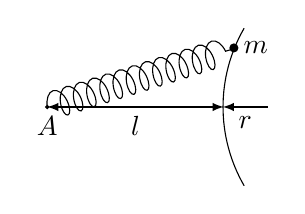
\begin{tikzpicture}
	\draw [arrows={latex-latex}] (0.5,0) -- (2.74,0) node [midway, below] {$l$};
	\draw (3.,1) arc (150:210:2);
	\draw [snake=coil, segment amplitude=5pt, segment length=5pt] (0.5,0) -- (2.9, 0.75);
	\draw [fill] (2.87, 0.75) circle (0.05) node [right] {$m$};
	\draw [fill] (0.5, 0) circle (0.02) node [below] {$A$};
	\draw [arrows={-latex}] (3.3,0) -- (2.73,0) node [midway, below ] {$r$};
\end{tikzpicture}
\end{document}